% !TEX root = ../main.tex
\subsubsection{Forward Detector} \label{sssec::forwarddetector}

% --+ HTCC +--------------------------------------------------------------------
\paragraph{High Threshold Cherenkov Counter (HTCC)}
    \begin{wrapfigure}{l}{0.50\textwidth}
        \centering\frame{
        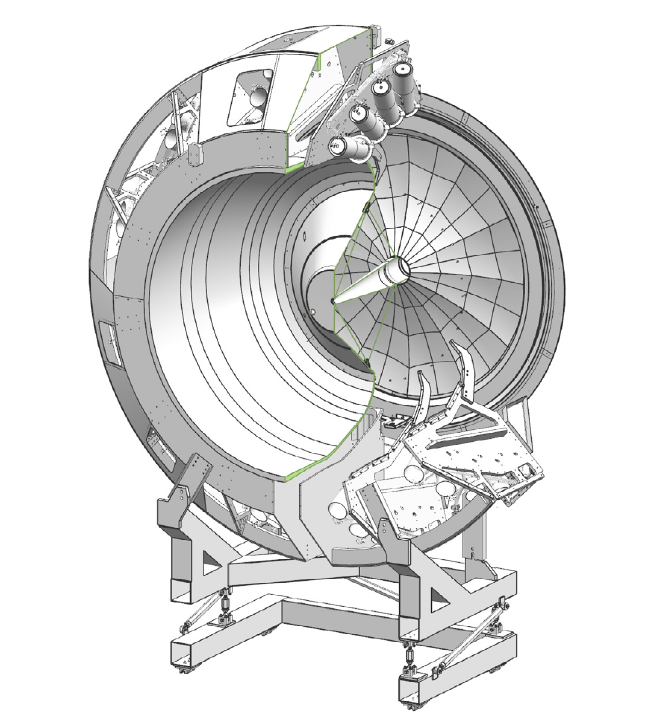
\includegraphics[width=\linewidth]{11experiment/img/21htcc.png}}
        \caption[HTCC]{Render of the High Threshold Cherenkov Counter.
        The container spans a diameter of about 4.5 m. The mirror is seen at the downstream end to the right.
        The PMTs are mounted in 12 sectors and in groups of 4 at the outer perimeter of the container.
        Light collection uses additional Winston cones and 5-in PMTs with quartz windows.}
        \label{fig::htcc}
    \end{wrapfigure}

    The HTCC is the main detector to separate electrons and positrons with momenta below 4.9 GeV from other charged particles.
    The detector has full azimuthal coverage and spans from $5\degree$ to $35\degree$ in polar angle.
    It has no blind areas in its complete solid angle coverage.
    The detector is located downstream of the target, fitted in between magnets, upstream of the forward tracking detectors.

    The HTCC system is mainly used for electron/positron identification, and thus it provides high rejection of charged pions and low background noise for reliable identification of scattered electrons in a dense electromagnetic background environment.
    The HTCC is a single unit operated in dry CO2 gas at 1 atm pressure.
    It is constructed using a multi-focal mirror of 48 elliptical mirror facets that focuses the Cherenkov light on 48 PhotoMultiplier Tubes (PMTs), each with a quartz window of 125 mm diameter.
    The PMTs are located in a magnetic field of up to $3.5\cdot 10^{-3}$ T oriented along the phototube axes and are surrounded along their lengths by a multi-layer magnetic shield with active compensation coils.

    In order to minimize multiple scattering in the HTCC detector materials and to limit its impact on the momentum analysis of charged tracks in the torus field, the HTCC mirror system is constructed using a backing structure of low-density composite material.
    As the detector is located in front of the momentum analysing torus magnet, all materials but the radiator gas in the path of the charged particles had to be kept to a minimum.
    In the actual detector, the density of the solid material seen by charged particles passing through the HTCC volume is $135 ~\text{mg}/\text{cm}^2$.
    The HTCC is also used to generate a fast signal to be used as a trigger for scattered electrons.
    The HTCC operates in conjunction with energy deposited in the electromagnetic calorimeters to identify electrons of specific energies \cite{sharabian2020}.
    A cut view of HTCC can be seen in Figure \ref{fig::htcc}.

% --+ DC +----------------------------------------------------------------------
\paragraph{Drift Chambers (DC)}
    \begin{wrapfigure}{r}{0.50\textwidth}
        \centering\frame{
        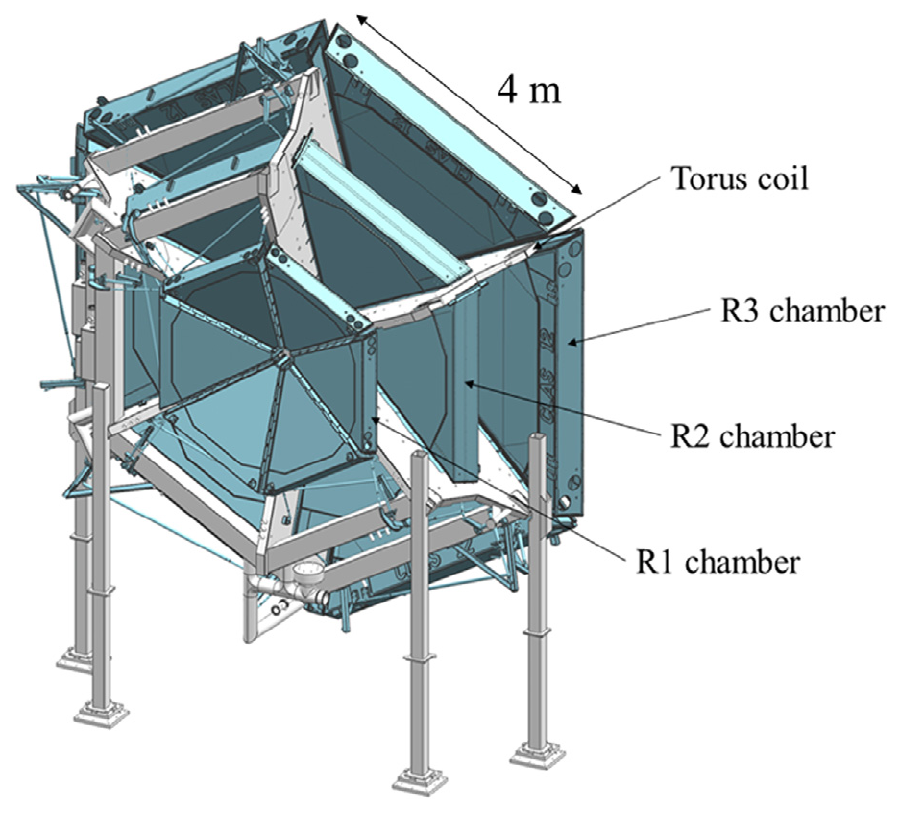
\includegraphics[width=\linewidth]{11experiment/img/21dc.png}}
        \caption[DC]{Drift Chambers render.
        Each of the DC regions are denoted as R1, R2, and R3 in the figure.}
        \label{fig::dc}
    \end{wrapfigure}

    The six coils of the torus magnet act as support for the forward tracking system, which consists of three independent drift chambers in each of the six sectors of the torus magnet.
    Each of the six DC sectors has a total of 36 layers with 112 sense wires each, arranged in three regions of twelve layers each.
    In each of the six torus sectors, the drift chambers are arranged identically.
    The arrangement of the DC around the torus coil can be seen in Figure \ref{fig::dc}

    As can be seen on the figure, the first region is located at the entrance to the torus magnetic field region.
    Then, the second is inside the magnet, where the magnetic field is close to its maximum.
    The third is located in a low magnetic field space, just downstream of the torus magnet.
    This arrangement provides independent and redundant tracking in each of the six torus sectors.

    Each of the three regions consists of six ``superlayers'', each of which contains two layers.
    One layer has wires strung at a stereo angle of $+6\degree$ while the second one of $-6\degree$, both with respect to the sector midplane.
    This stereo view enables excellent resolution in the polar angle ($\Delta\theta < 2 ~\text{mrad}$), and good resolution in the azimuthal scattering angle ($\Delta\phi < 2 ~\text{mrad}$).

    The DC can detect ionising particles with momenta above $200 ~\text{MeV}/\text{c}$, with a $\Delta p/p$ lesser than $0.5\%$.
    This offers a track momentum resolution of $3$ to $5\%$ \cite{mestayer2020}.

% --+ LTCC +--------------------------------------------------------------------
\paragraph{Low Threshold Cherenkov Counter (LTCC)}
    The LTCC system is used for charged pion and kaon detection at momenta between $3.5$ and $9 ~\text{GeV}$.
    The LTCC system consists of boxes shaped like truncated pyramids.
    Four of the six sectors of CLAS12 are equipped with one LTCC box.
    Each LTCC box contains 108 lightweight mirrors with composite backing structures, 36 Winston light-collecting cones, 36 125-mm diameter PMTs, and 36 magnetic shields.
    The LTCC boxes are filled with heavy C4 F10 radiator gas.

    \begin{wrapfigure}{l}{0.50\textwidth}
        \centering\frame{
        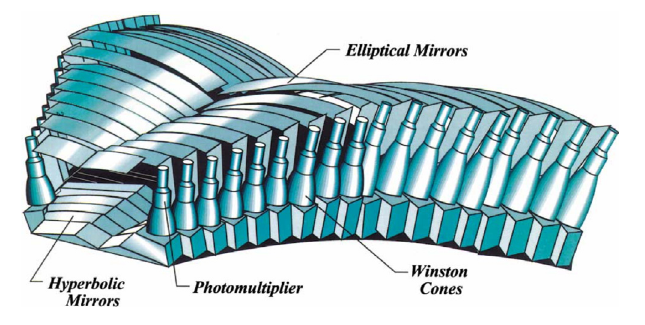
\includegraphics[width=\linewidth]{11experiment/img/21ltcc.png}}
        \caption[LTCC Mirror System]{Layout and components of the optical mirror system within each LTCC box from the design model.}
        \label{fig::ltcc}
    \end{wrapfigure}

    The LTCC was a detector used in CLAS, which as part of the 12 GeV upgrade was refurbished to provide higher efficiency for charged pion and kaon detection.
    This was done by increasing the volume of the radiator gas, refurbishing the elliptical and hyperbolic mirrors with new coatings, and improving the sensitivity of the PMTs to Cherenkov light.
    The sensitivity improvement was achieved by coating their entrance windows with wavelength shifting material that absorbs ultraviolet (UV) light at wavelength below $300 ~\text{nm}$ and re-emits two back-to-back photons at larger wavelength \cite{ungaro2020}.
    A drawing from the design model of the LTCC can be seen in Figure \ref{fig::ltcc}.

% --+ FTOF +--------------------------------------------------------------------
\paragraph{Forward Time-of-Flight (FTOF)}
    \begin{wrapfigure}{r}{0.50\textwidth}
        \centering\frame{
        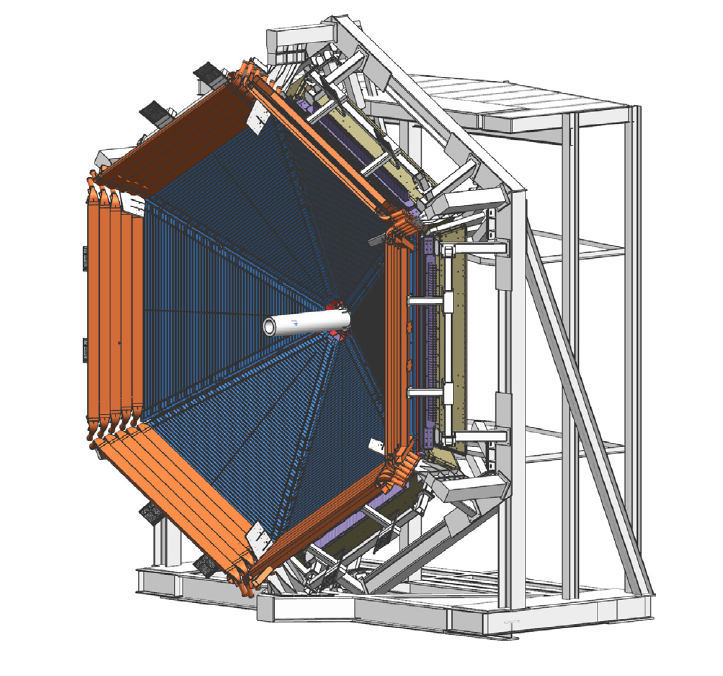
\includegraphics[width=\linewidth]{11experiment/img/21ftof.png}}
        \caption[FTOF]{Render of the Forward Carriage with the FTOF system showing the panel-1b counters on the inside (dark blue), and the panel-2 counters on the outside (bronze).
        The panel-1a counters are located immediately downstream of the panel-1b counters and are not visible in the render.
        Part of the PCAL is visible downstream of the FTOF panels.}
        \label{fig::ftof}
    \end{wrapfigure}

    The FTOF system is used to measure the TOF of charged particles emerging from the target during beam operation.
    It includes six sectors of plastic scintillators with double-sided PMT readout.
    Each sector consists of three arrays of counters separated in panels, with panel-1a having 23 counters, panel-1b 62 counters, and panel-2 5 counters.
    The system is required to get excellent timing resolution required for particle identification and good segmentation to get flexible triggering options.

    The detectors span a range in polar angle from $5\degree$ to $45\degree$, covering $50\%$ in the azimuth at $5\degree$ and $90\%$ at $45\degree$.
    The lengths of the counters range from $32.3 ~\text{cm}$ to $376.1 ~\text{cm}$ in panel 1a, from $17.3 ~\text{cm}$ to $407.9 ~\text{cm}$ in panel-1b, and from $371.3 ~\text{cm}$ to $426.2 ~\text{cm}$ in panel-2.
    The average timing resolution in panel-1a is $125 ~\text{ps}$, $85 ~\text{ps}$ in panel-1b, and $155 ~\text{ps}$ in panel-2 \cite{carman2020ftof}.
    A render of the detector can be seen in Figure \ref{fig::ftof}.

% --+ RICH +--------------------------------------------------------------------
\paragraph{Ring Imaging Cherenkov Detector (RICH)}
    For momenta greater than 3 GeV, the TOF resolution of FTOF is not sufficient to separate kaons from pions.
    For that puspose, an additional RICH detector was built and incorporated into one of the CLAS12 sectors to replace the corresponding LTCC sector.
    The RICH detector is designed to improve CLAS12 particle identification in the momentum range $3 - 8 ~\text{GeV}$.
    The detector incorporates aerogel radiators, visible light photon detectors, and a focusing mirror system that is used to reduce the detection area instrumented by photon detectors to $1 ~\text{m}^2$.

    Multi-anode PhotoMultiplier Tubes (MaPMTs) provide the required spatial resolution and match the aerogel Cherenkov light spectrum in the visible and near-UV region.
    For forward scattered particles up to $13\degree$ with momenta $3 - 8 ~\text{GeV}$, a proximity imaging method with thin ($2 ~\text{cm}$) aerogel and direct Cherenkov light detection is used.
    For larger incident particle angles between $13\degree$ and $25\degree$ and momenta of $3 - 6 ~\text{GeV}$, the Cherenkov light is produced by a thicker aerogel layer of $6 ~\text{cm}$, focused by a spherical mirror, and undergoes two further passes through the thin radiator material and a reflection from planar mirrors before detection \cite{contalbrigo2020}.

% --+ ECAL +--------------------------------------------------------------------
\paragraph{Electromagnetic Calorimeters (ECAL)}
    The CLAS12 detector package uses the existing electromagnetic calorimeter (EC) of the CLAS detector, but adds to it a new pre-shower calorimeter (PCAL), which is installed upstream of the EC.
    Together, the PCAL and EC are referred to as the ECAL.
    The calorimeters in CLAS12 are used primarily for the identification and kinematical reconstruction of electrons, photons, and neutrons.

    The PCAL and EC are both sampling calorimeters consisting of six modules.
    Along the direction from the target, the EC consists of two parts, read out separately, called EC-inner (ECIN) and EC-outer (ECOU).
    They provide longitudinal sampling of electromagnetic showers, as well as of hadronic interactions to improve particle identification.
    Each module has a triangular shape with 54 (15/15/24, PCAL/ECIN/ECOU) layers of 1-cm-thick scintillators segmented into 4.5/10-cm (PCAL/EC) wide strips fitted between 2.2-mm-thick lead sheets.
    The total thickness corresponds to approximately 20.5 radiation lengths.
    Scintillator layers are grouped into three readout views with 5/5/8 PCAL/ECIN/ECOU layers per view, providing spatial resolutions of less than $2 ~\text{cm}$ for energy clusters.
    The light from each scintillator readout group is routed to the PMTs via flexible optical fibres \cite{asryan2020}.

% --+ FT +----------------------------------------------------------------------
\paragraph{Forward Tagger (FT)}
    The FT extends the capabilities of CLAS12 to detect electrons and photons at the very forward polar angles from $2.5\degree$ to $4.5\degree$.
    The detection of forward-going scattered electrons allows for electroproduction experiments at very low photon virtuality $Q^2$, providing an energy-tagged, linearly polarized, high-intensity, quasi-real photon beam.
    This configuration enables execution of an extensive hadron spectroscopy program.

    \begin{wrapfigure}{l}{0.50\textwidth}
        \centering\frame{
        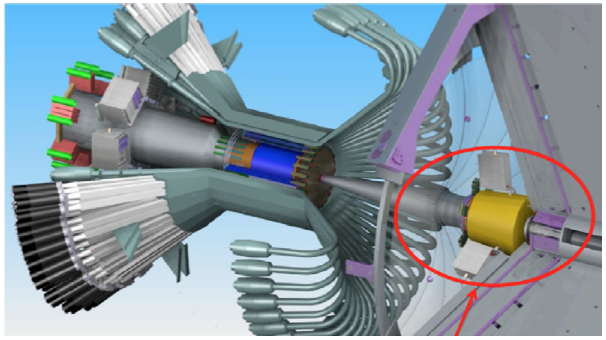
\includegraphics[width=\linewidth]{11experiment/img/21ft.png}}
        \caption[FT]{The Forward Tagger system circled downstream of the CD in front of the torus magnet warm bore entrance.}
        \label{fig::ft}
    \end{wrapfigure}

    The FT consists of a calorimeter (FTCal), a micro-strip gas tracker (FTTrk), and a hodoscope (FTHodo).
    The FTCal with 332 lead-tungstate ($\text{PbWO}_4$) crystals is used to identify electrons, measure the electromagnetic shower energy, and provide a fast trigger signal.
    The FTTrk in front of it measures the charged particle scattering angles.
    The scintillator FTHodo aids in separating electrons and high-energy photons.

    During beam operations, a tungsten shielding pipe of conical shape is installed in front of the FT to absorb M\o ller electrons and low-energy photons produced by beam interactions with the target and downstream materials.
    This shield protects both the FT and the Forward Detectors from electromagnetic background.
    The cone angle is $2.5\degree$, such that it is compatible with the FT acceptance.
    In this configuration, known as ``FT-ON'', the FT can be used to detect both electrons and photons, extending the detection capabilities of CLAS12.

    \begin{wrapfigure}{r}{0.50\textwidth}
        \centering\frame{
        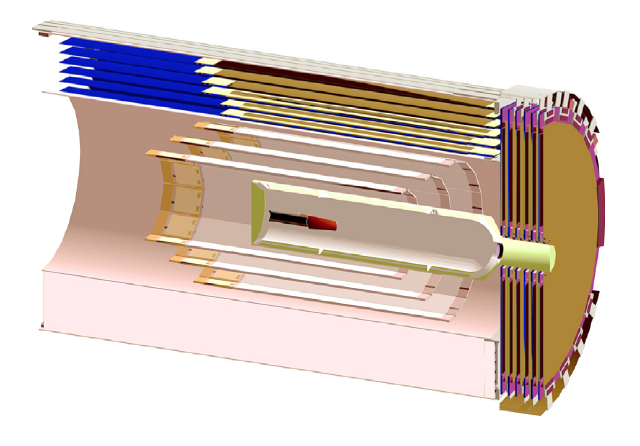
\includegraphics[width=\linewidth]{11experiment/img/22cvt.png}}
        \caption[CVT]{Render of the Central Vertex Tracker.
        From the inside, the figure shows the target cell and vacuum chamber, the three double layers of the SVT, followed by the six layers of the BMT.
        The beam enters from the left.
        The six FMT layers are shown at the downstream end at the right.}
        \label{fig::cvt}
    \end{wrapfigure}

    Alternatively, when the FT is not needed for the physics program, the FT detectors are turned off and additional shielding elements are installed in front of the FT covering up to $4.5\degree$ to reduce the background in the DC R1 chambers.
    This configuration, known as ``FT-Off'', reduces the accidental background by one-third at the same beam conditions, which allows for higher luminosity data taking with CLAS12 \cite{acker2020ft}.
    A render of the CD with the FT circled can be seen in Figure \ref{fig::ft}.
